
\subsection{LM-band imaging}
\label{ssec:recipes_img_lm}

\subsubsection{LM-band imaging flatfield}
\label{lm_img_flatfield}
\label{rec:lm_img_flatfield}
\label{sssec:lm_img_flatfield}
\label{metis_lm_img_flat}
\label{rec:metis_lm_img_flat}
\label{sssec:metis_lm_img_flat}

The purpose of the flat-field calibration is to determine
pixel-to-pixel gain variations and large scale illumination variations
(due to inhomogeneities of optical elements in the telescope or
instrument). Calibration frames are obtained either during day time
using the black-body lamp of the \ac{WCU} (internal flats) or by taken
images of the twilight sky (twilight flats). Advantages and
disadvantages of the two types of flat are discussed in
\cite{METIS-calibration_plan}. Since the operational concept for
twilight flats needs to be refined during commissioning at the
telescope, the current recipe design is primarily valid for internal
flats.

This recipe creates a master flat for the HAWAII2RG detector (LM-band
imaging) from lamp or sky images matched by various setup parameters
as detailed below.  A set of internal flats includes a number of
exposures with \CODE{LAMP OFF}, which will be used for dark
subtraction. For twilight flats a master dark will be subtracted. The
master flat is obtained by the slope of a linear fit of the pixel
values against the illumination level of the exposures.

The quality control parameters give various statistics for each input
frame (mean, standard deviation, etc.), the standard deviation of the
normalised master flat and the number of bad pixels identified by the
recipe. If a bad-pixel map is provided on input, it is updated,
otherwise a new one is created.

\begin{recipedef}
  Name:                & \REC{metis_lm_img_flat}                                        \\
  Purpose:             & Create master flat field for the LM-band imaging detector.     \\
  Requirements:        & \REQ{METIS-6096}                                               \\
  Type:                & Calibration                                                    \\
  Templates:           & \TPL{METIS_img_lm_cal_InternalFlat}                            \\
                       & \TPL{METIS_img_lm_cal_TwilightFlat}                               \\
  Input data:          & Flat field images taken with lamp or sky.                      \\
                       & Master dark (for twilight flats)                               \\
                       & Bad pixel map                                                  \\
  Matched keywords:    & Detector ID                                                    \\
                       & Filter ID                                                      \\
                       & ADC ID                                                         \\
                       & Flat type (internal or twilight)                               \\
                       & possibly others (e.g.\ coronagraphic mask, \TBD)               \\
  Parameters:          & Combination method (\texttt{mean}, \texttt{median},
                         \texttt{sigclip}, \dots)                                       \\
                       & Parameters for combination methods                             \\
                         & Threshold(s) for deviant-pixel identification                  \\
 Algorithm:            & Call \REC{metis_apply_persistance_correction} to apply the persistance correction \\
                         & For internal flats: call \REC{metis_det_dark} with \CODE{LAMP OFF} images to create dark frame. \\
 & Subtract internal dark or master dark from flat exposures.     \\
  & call \REC{metis_lm_img_flat} to fit slope of pixel values against illumination level. Frames
  with the same exposure time will be averaged.\\
                       & Compute median or average of input frames to improve statistics.\\
                       & Call \REC{metis_update_lm_flat_mask} to flag deviant pixels. \\
  Output data:         & \PROD{MASTER_IMG_FLAT_2RG}                                     \\
                       & \PROD{BADPIX_MAP_2RG}                                          \\
  Expected accuracies: & \TBD                                                           \\
  QC1 parameters:      & \QC{QC LM MASTERFLAT RMS}                                      \\
                       & \QC{QC LM FLAT NBADPIX}                                        \\
                       & \QC{QC LM FLAT MEAN ##}                                        \\
                       & \QC{QC LM FLAT RMS ##}                                         \\
  hdrl function:       & \CODE{hdrl_bpm_fit_compute}                                    \\
                       & \CODE{hdrl_imagelist_collapse} \\
                       & \CODE{hdrl_imagelist_sub_image}                                \\
\end{recipedef}

\begin{figure}[hb]
  \centering
  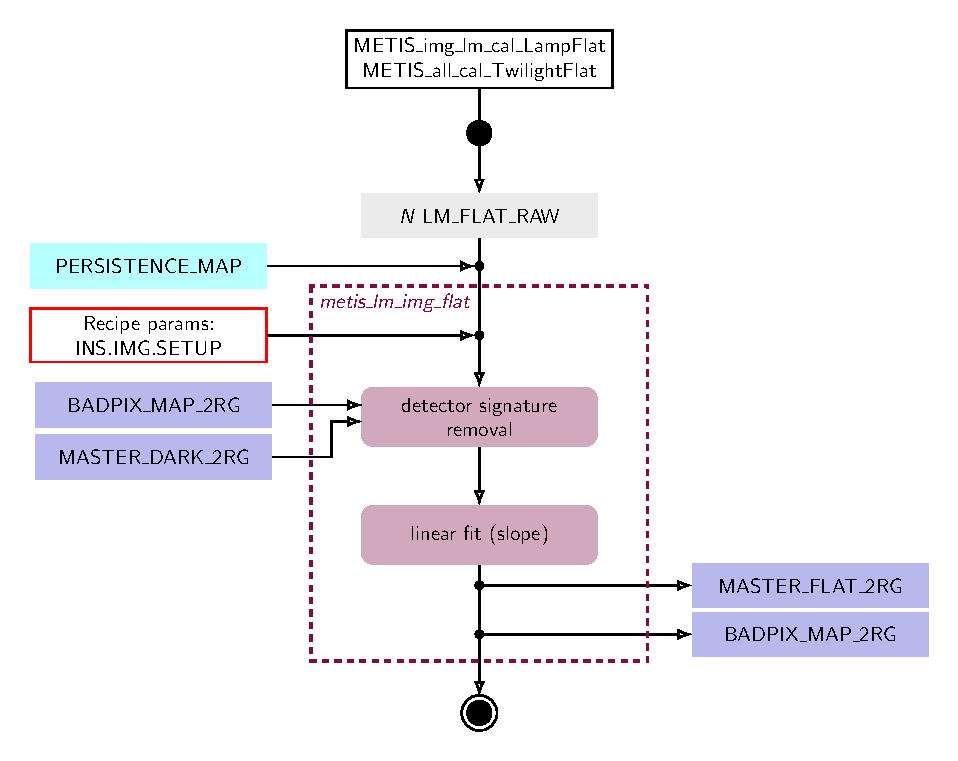
\includegraphics[width=0.6\textwidth]{metis_lm_img_flat}
  \caption[Recipe: \REC{metis_lm_img_flat}]{\REC{metis_lm_img_flat} --
    creation of \CODE{IMG_LM} master flatfield.\\ \TODO{Include averaging of
      frames at same illumination}}
  \label{fig:metis_lm_img_flat}
\end{figure}


\clearpage
\subsubsection{LM-band imaging basic reduction}
\label{lm_img_basic}
\label{rec:lm_img_basic}
\label{sssec:lm_img_basic}
\label{metis_lm_img_basic_reduce}
\label{rec:metis_lm_img_basic_reduce}
\label{sssec:metis_lm_img_basic_reduce}

\TODO{New recipe -- this may be too basic and could be joined with
  the background subtraction.}

This recipe performs the basic reduction of raw exposures from the
LM-band imager, i.e.\ dark subtraction, flat fielding and other removing
instrumental signals. It is used for both standard and science exposures.

Basic statistics of the images can be used to screen for saturation.

\TODO{This recipe should analyse the masked detector regions for
  channel offset correction and crosstalk (see \cite{matisse_minutes}).}

\begin{recipedef}
  Name:             & \REC{metis_lm_img_basic_reduce}   \\
  Purpose:          & apply basic reduction of images   \\
  Type:             & Calibration, Science              \\
  Templates:        & \TPL{METIS_img_lm_cal_standard}  \\
                    & \TPL{METIS_img_lm_*_obs_*}       \\
  Input data:       & Dithered images (standard, science) \\
                    & Blank sky images (if available)   \\
                    & Masked detector region (if available)  \\
                    & Master dark                       \\
                    & Master flat                       \\
  Matched keywords: & DIT (for dark)                    \\
                    & Filter ID (for flat)              \\
  Algorithm:        & Remove crosstalk, correct non-linearity \\
                    & Analyse and remove masked regions  \\
                    & Subtract dark, divide by flat       \\
                    & Remove blank sky pattern                \\
  Output data:      & \PROD{LM_SCI_BASIC_REDUCED}       \\
                    & \PROD{LM_STD_BASIC_REDUCED}       \\
  QC1 parameters:   & \QC{QC LM IMG MEDIAN}             \\
                    & \QC{QC LM IMG STANDARD DEVIATION} \\
                    & \QC{QC LM IMG PEAK}               \\
  hdrl functions:   & \CODE{hdrl_imagelist_sub_image}   \\
                    & \CODE{hdrl_imagelist_div_image}   \\
\end{recipedef}

\begin{figure}[hb]
  \centering
  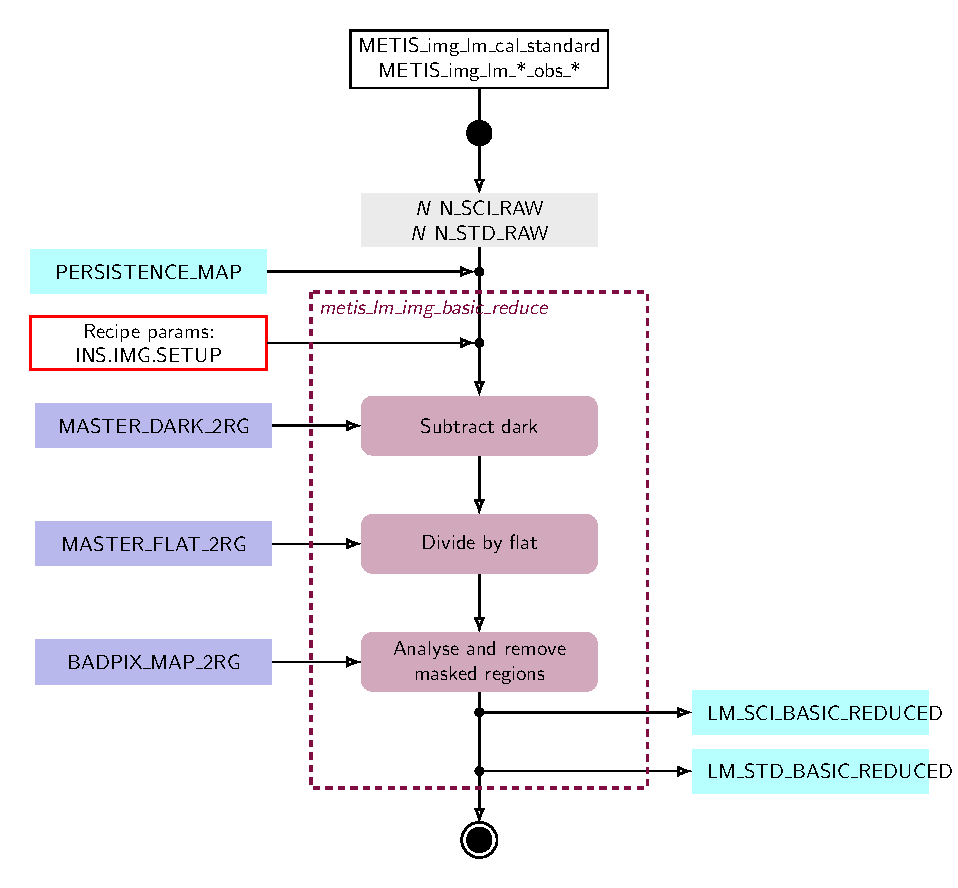
\includegraphics[width=0.6\textwidth]{metis_lm_img_basic_reduce}
  % \resizebox{0.6\textwidth}{0.1\textwidth}{\TODO{\fbox{Figure to be done}}}
  \caption[Recipe: \REC{metis_lm_img_basic_reduce}]{\REC{metis_lm_img_basic_reduce} --
    basic reduction of \CODE{IMG_LM} data.}
  \label{fig:metis_lm_img_basic_reduce}
\end{figure}


\clearpage
\subsubsection{LM-band imaging background subtraction}
\label{lm_img_background}
\label{rec:lm_img_background}
\label{sssec:lm_img_background}
\label{metis_lm_img_background}
\label{rec:metis_lm_img_background}
\label{sssec:metis_lm_img_background}

This recipe estimates and subtracts the background from LM-band
imaging data. Thermal background emission from the atmosphere,
telescope and warm parts of the instrument dominate the photon count
in mid-infrared observations. Accurate determination and removal of
background counts is therefore crucial to make MIR data scientifically
usable.

A set of observations will consist of a number of dithered exposures
of the field, where the offsets are achieved using the internal
chopper of METIS or the with the telescope. For extended objects, the
telescope will be used to perform ``out-of-field dithering'', i.e.\
observe nearby blank patches of sky interlaced with the target
observations. Imaging observations are performed in pupil-tracking
mode, hence angular dithering of the field is automatic.

For in-field-dithered exposures, all dithered exposures will be
averaged to obtain the background estimate. In order to only average
the background contribution, an iterative procedure of object
detection and masking will be employed. Averaging will be done using a
robust estimator of the mean (e.g.\ median).

For extended objects, all out-of-field exposures will be averaged
(with object rejection) and subtracted off the in-field exposures.

\TODO{Object catalogues of the target exposures could be created within this
recipe or in a separate recipe. The catalogue should contain for each
object: pixel coordinates ($x$, $y$), world coordinates ($\alpha$,
$\delta$) based on telescope pointing and derotator information, total
counts within an aperture.}

\TODO{Is this good enough for HCI images or do we need more?}

\begin{recipedef}
  Name:             & \REC{metis_lm_img_background}                             \\
  Purpose:          & estimate and subtract background                          \\
  Type:             & Calibration                                               \\
  Templates:        & \TPL{METIS_img_lm_cal_standard}                           \\
                    & \TPL{METIS_img_lm_*_obs_*}                                \\
  Input data:       & \CODE{LM_SCI_BASIC_REDUCED}                               \\
                    & \CODE{LM_STD_BASIC_REDUCED}                               \\
  Matched keywords: & dither position (\CODE{SKY}? \TBD)                        \\
  Algorithm:        & Average all or \CODE{SKY} exposures with object rejection \\
                    & Subtract background                                       \\
  Output data:      & \PROD{LM_SCI_BKG}                                         \\
                    & \PROD{LM_STD_BKG}                                         \\
                    & \PROD{LM_SCI_BKG_SUBTRACTED}                              \\
                    & \PROD{LM_STD_BKG_SUBTRACTED}                              \\
                    & \PROD{LM_SCI_OBJECT_CAT}                                  \\
                    & \PROD{LM_STD_OBJECT_CAT}                                  \\
  QC1 parameters:   & \QC{QC LM IMG BKG MEDIAN}                                 \\
                    & \QC{QC LM IMG BKG MEDIAN DEVIATION}                       \\
  hdrl functions:   & \CODE{hdrl_imagelist_sub_image}                           \\
                    & \CODE{hdrl_imagelist_div_image}                           \\
                    & \CODE{hdrl_catalogue_compute}                             \\
\end{recipedef}

\begin{figure}[hb]
  \centering
  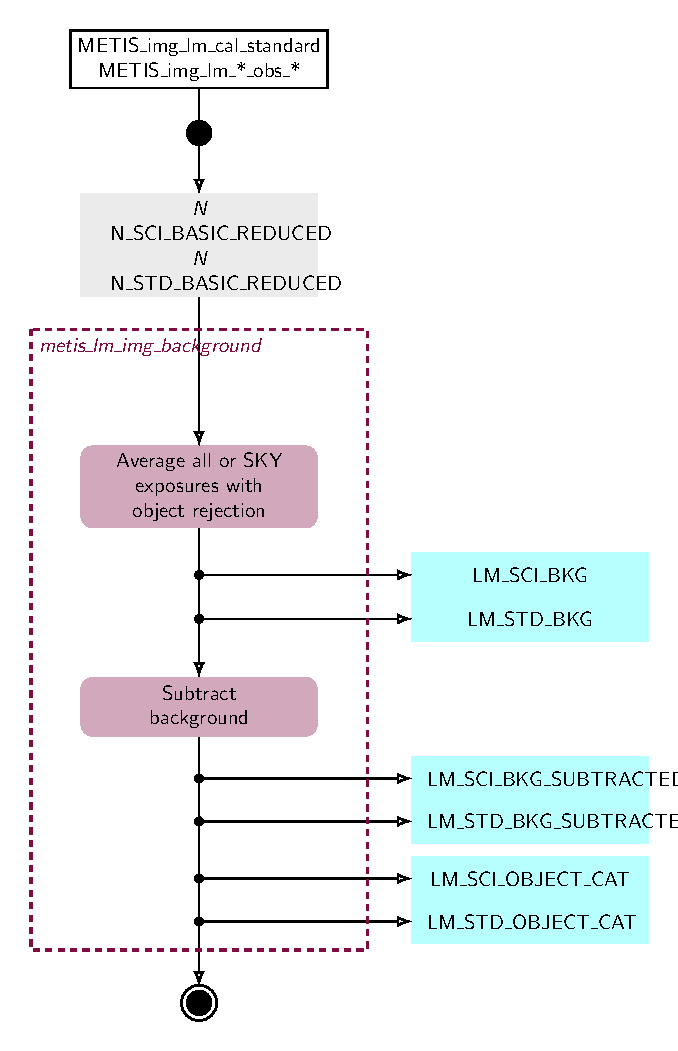
\includegraphics[width=0.6\textwidth]{metis_lm_img_background}
  % \resizebox{0.6\textwidth}{0.1\textwidth}{\TODO{\fbox{Figure to be done}}}
  \caption[Recipe: \REC{metis_lm_img_background}]{\REC{metis_lm_img_background} --
    background estimation and subtraction of dithered \CODE{IMG_LM} data.}
  \label{fig:metis_lm_img_background}
\end{figure}


\clearpage

\subsubsection{LM-band imaging astrometry calibration}
\label{lm_img_astrometry_calib}
\label{rec:lm_img_astrometry_calib}
\label{sssec:lm_img_astrometry_calib}
\label{metis_lm_img_astrometry_process}
\label{rec:metis_lm_img_astrometry_process}
\label{sssec:metis_lm_img_astrometry_process}
This recipe is the conversion of the pixel coordinates (X,Y) of objects in an image
into their corresponding celestial coordinates of right ascension (RA) and 
declination (Dec). The recipe for astrometry calibration involves several 
steps that must be carried out precisely to achieve accurate results.

The first step of the recipe involves identifying a set of reference stars 
in the image, whose coordinates are well known and can be obtained from a 
catalog. This requires careful selection and verification of the reference stars, 
as their accuracy determines the accuracy of the final calibration.

The next step is to use these reference stars to establish a mapping between 
the image's pixel coordinates and their corresponding celestial coordinates. This 
is achieved through a process called plate solving, which involves solving a set 
of mathematical equations to determine the transformation between pixel and celestial 
coordinates. This process requires careful selection of the appropriate transform function 
and calibration parameters.

\begin{recipedef}
  Name:                & \REC{metis_lm_img_astrometry_process}                                               \\
  Purpose:             & Determine conversion factor between pixel and world coordinates              \\
  Type:                & Calibration                                                                  \\
  Templates:           & \TPL{METIS_img_lm_cal_standard}                                              \\
  Input data:          & \CODE{LM_STD_BKG_SUBTRACTED}                                                 \\
                       & photometric standard catalogue                                               \\
  Matched keywords:    & OBJECT ID                                                                    \\
                       & FILTER ID                                                                    \\
  Parameters:          & Distortion correction functions                                              \\
  Algorithm:           & Measure position of stars in pixel coordinates                               \\
                       & Compute conversion factor to world coordinates                               \\
                       & Measure and evaluate the error.                                              \\
  Output data:         & \PROD{LM_STD_AST_CALIB}                                                      \\
                       & \PROD{ASTROMETRY_TAB}                                                        \\
  Expected accuracies: &  $>$0.1$\arcsec$                                                                    \\
  QC1 parameters:      & \QC{QC LM AST X POS ERR}                                                     \\
                       & \QC{QC LM AST Y POS ERR}                                                     \\
                       & \QC{QC LM AST RA POS ERR}                                                    \\
                       & \QC{QC LM AST DEC POS ERR}                                                    \\
  hdrl function:       & \CODE{hdrl_strehl_compute}                                                   \\
                       & \CODE{hdrl_catalogue_compute}                                                \\
                       & \CODE{hdrl_efficiency_compute}                                               \\
                       & \CODE{hdrl_imagelist_collapse}                                               \\
\end{recipedef}

\begin{figure}[hb]
  \centering
   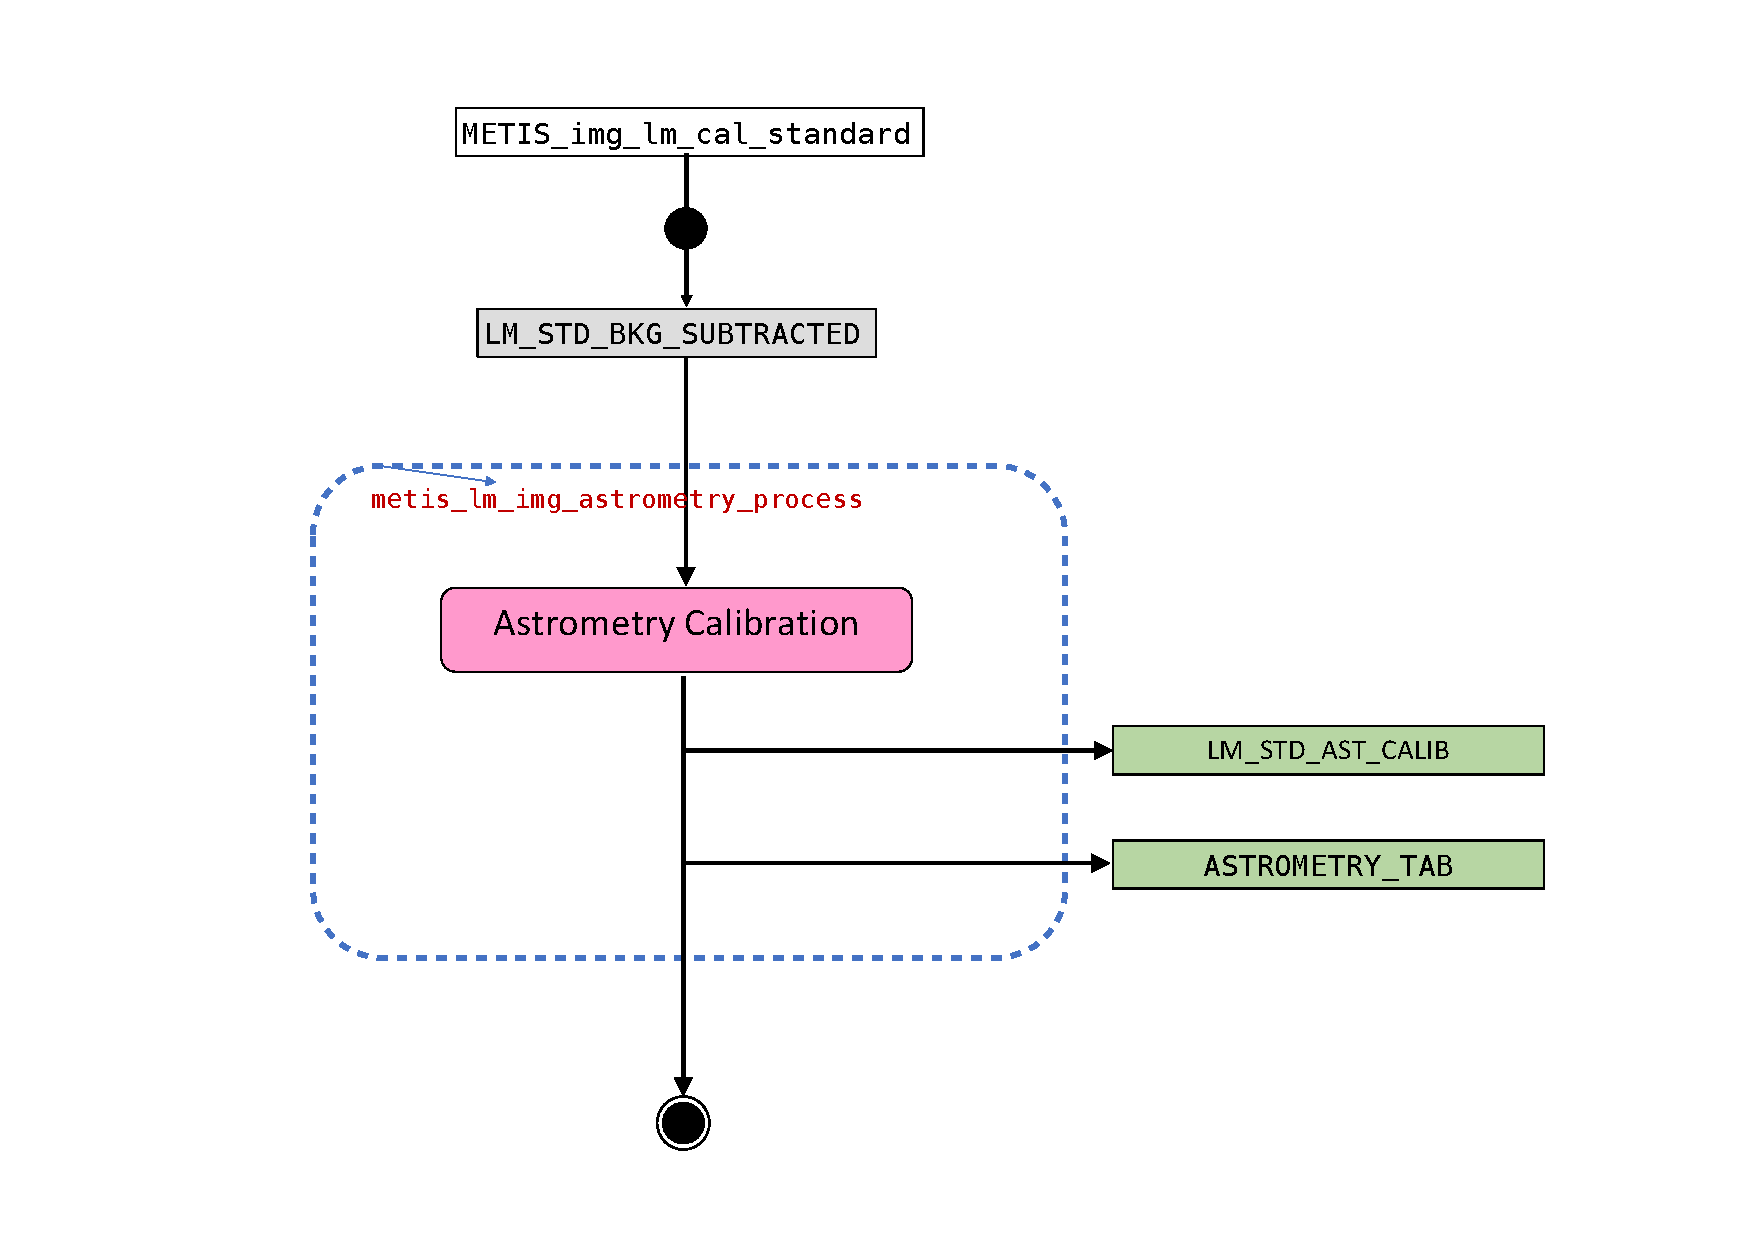
\includegraphics[width=1.0\textwidth]{metis_lm_img_astrometry_process}
  %\resizebox{0.6\textwidth}{0.1\textwidth}{\TODO{\fbox{Figure to be done}}}
  \caption[Recipe: \REC{metis_lm_img_astrometry_process}]{\REC{metis_lm_img_astrometry_process} --
    compute conversion between pixel and sky coordinate}
  \label{fig:metis_lm_img_astrometry_process}
\end{figure}


\clearpage

\subsubsection{LM-band imaging photometric standard analysis}
\label{lm_img_photstd}
\label{rec:lm_img_photstd}
\label{sssec:lm_img_photstd}

This recipe determines the conversion from ADU to physical units from
a set of reduced exposures of a photometric standard star. The flux of
the star is measured in each exposure in ADU, normalised to an
exposure time of 1~second and averaged over all exposures. In
addition, the exposures are stacked (after recentering on the standard
star, but without derotation) and the flux is measured in the combined
image. Comparison to the tabulated brightness of the star in the
observing filter yields the conversion factor from
$\mathrm{ADU\,s^{-1}}$ to $\mathrm{photons\,\,s^{-1}\,cm^{-2}}$.

QC parameter will include estimates of the sensitivity for the
detection of point sources and surface brightness sensitivity
following \cite{visir_manual}.

\begin{recipedef}\label{rec:metis_lm_img_std_process}
  Name:                & \REC{metis_lm_img_std_process}                                               \\
  Purpose:             & Determine conversion factor between detector counts and physical source flux \\
  Type:                & Calibration                                                                  \\
  Templates:           & \TPL{METIS_img_lm_cal_standard}                                              \\
  Input data:          & \CODE{LM_STD_AST_CALIB}                                                 \\
                       & photometric standard catalogue                                               \\
  Matched keywords:    & OBJECT ID                                                                    \\
                       & FILTER ID                                                                    \\
  Parameters:          & None (TBD)                                                                   \\
  Algorithm:           & Call \REC{calculate_std_flux} to measure flux in input images                      \\
                       & call \REC{recentre_img} to recentre and stack images                         \\
                       & call \REC{calculate_std_flux} on the stacked image to get flux of the star in detector units\\
                       & call \REC{caluculate_std_fluxcal} to calculate the conversion factor to physical units    \\
                       & call \REC{calculate_detection_limits} to compute measure background noise (std,rms) and compute detection limits \\
  Output data:         & \PROD{LM_STD_COMBINED}                                                       \\
                       & \PROD{FLUXCAL_TAB}                                                           \\
  Expected accuracies: & \TBD                                                                         \\
  QC1 parameters:      & \QC{QC LM IMG STD BACKGD RMS}                                                \\
                       & \QC{QC LM STD PEAK CNTS}                                                     \\
                       & \QC{QC LM STD APERTURE CNTS}                                                 \\
                       & \QC{QC LM STD STREHL}                                                        \\
                       & \QC{QC LM STD FLUXCONV}                                                      \\
                       & \QC{QC LM STD AIRMASS}                                                       \\
                       & \QC{QC LM SENSITIVITY}                                                       \\
                       & \QC{QC LM AREA SENSITIVIY}                                                   \\
  hdrl function:       & \CODE{hdrl_strehl_compute}                                                   \\
                       & \CODE{hdrl_catalogue_compute}                                                \\
                       & \CODE{hdrl_efficiency_compute}                                               \\
                       & \CODE{hdrl_imagelist_collapse}                                               \\
\end{recipedef}

\begin{figure}[hb]
  \centering
   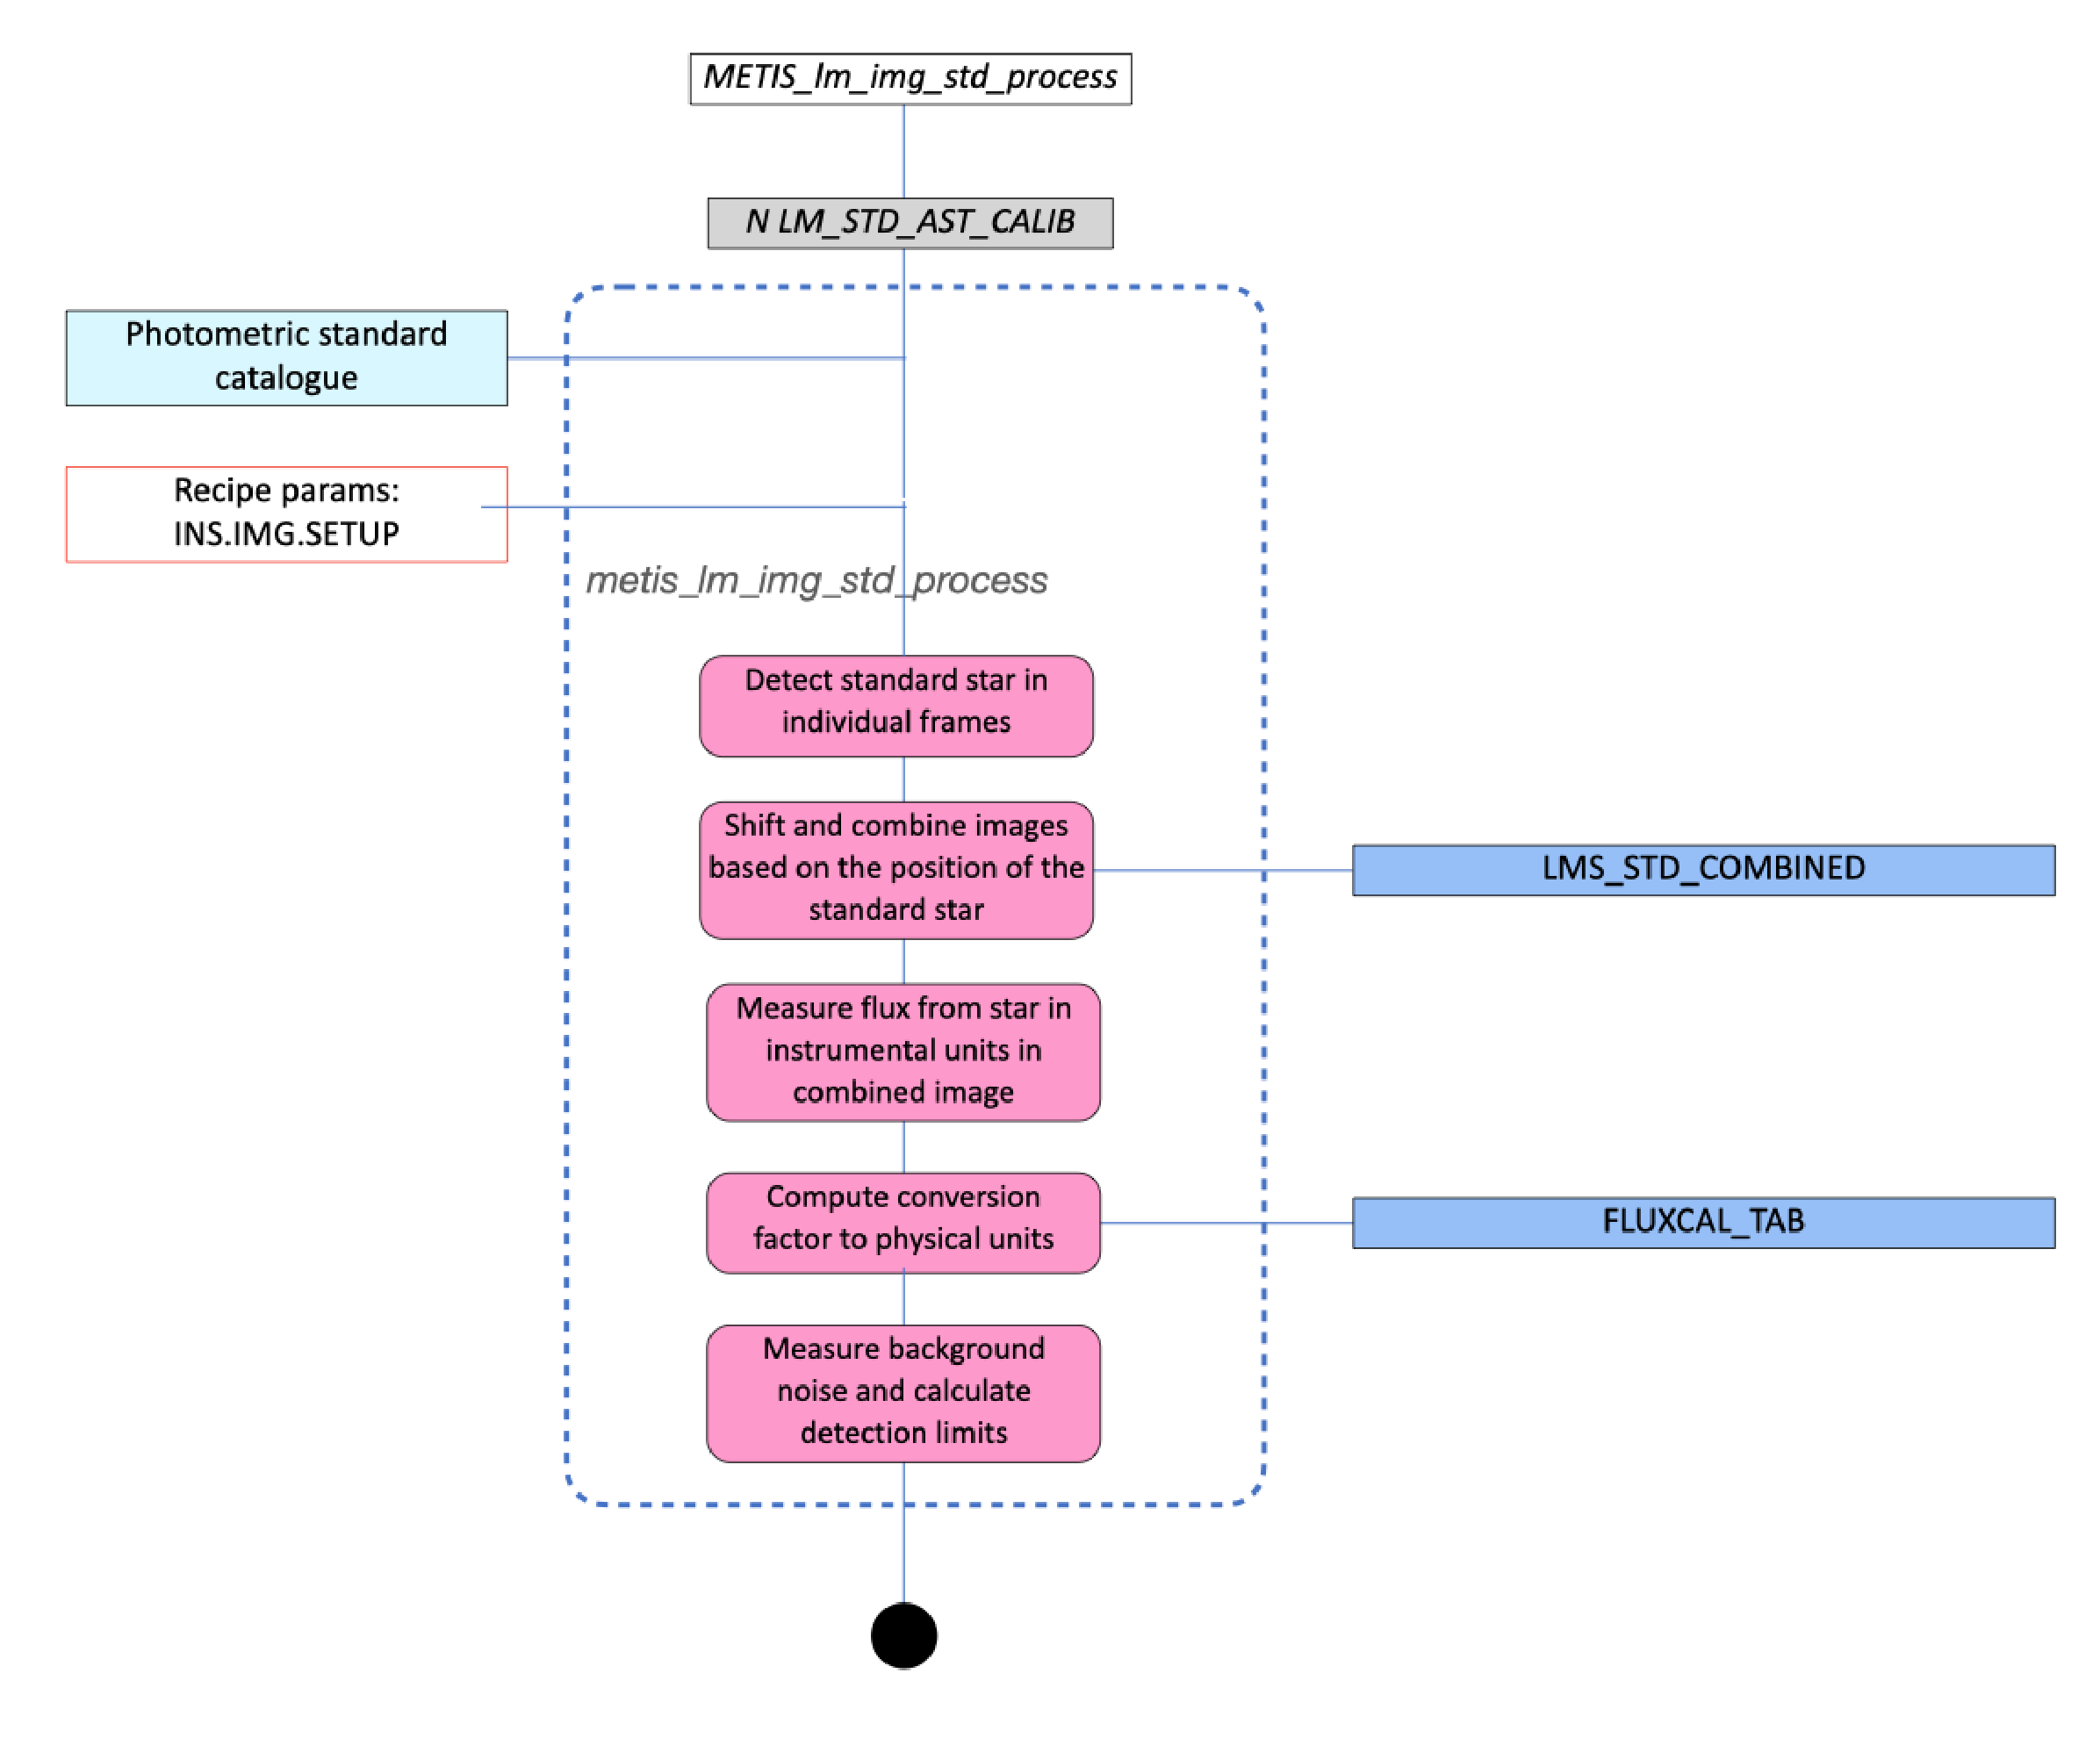
\includegraphics[width=0.6\textwidth]{metis_lm_img_std_process}
  %\resizebox{0.6\textwidth}{0.1\textwidth}{\TODO{\fbox{Figure to be done}}}
  \caption[Recipe: \REC{metis_lm_img_std_process}]{\REC{metis_lm_img_std_process} --
    compute conversion between ADU and physical flux units}
  \label{fig:metis_lm_img_std_process}
\end{figure}

%%%%%%%%%%%%%%%%%%%%%%%%%%%%%%%%%%%%%%%%%%%%%%%%%

\clearpage
\subsubsection{LM-band imaging calibration}
\label{lm_img_calibrate}
\label{rec:lm_img_calibrate}
\label{sssec:lm_img_calibrate}

This recipe applies the flux calibration to the reduced science
images and adds geometric calibration data to the FITS header. The
products of this recipe are fully calibrated individual exposures.

Each image is multiplied by the conversion factor such that pixel
values are in units of photons per second per centimetre squared. The
header of each file receives keyword \FITS{BUNIT} with value %
\CODE{'photon.s**(-1).cm**(-2)'}.

\TODO{Other units may be possible, although additional information is
  needed. For instance,\\ \CODE{'photon.s**(-1).cm**(-2).arcsec**(-2)'} makes
  values independent of the pixel scale, but requires a distortion map
  (variation of pixel scale across the detector). Energy units (erg
  instead of photons) require knowledge of the spectral energy
  distribution of the sources, in particular for broad-band filters.}

LM-band imaging observations will be performed in pupil-tracking mode
\cite{METIS-operational_concept}, which means that the field rotates
from exposure to exposure.  The information about the field
orientation along with target coordinates, pixel scale and
higher-order polynomial distortion coefficients is written to the FITS
header. The images are not resampled by this recipe, this is left to
\REC{metis_lm_img_sci_postprocess}.



\begin{recipedef}\label{rec:metis_lm_img_calibrate}
  Name:              & \REC{metis_lm_img_calibrate}                     \\
  Purpose:           & Convert science images to physical units         \\
                     & Add distortion information                       \\
  Type:              & Calibration                                      \\
  Templates          & ??                                                 \\
  Input data:        & \PROD{LM_SCI_BKG_SUBTRACTED}                     \\
                     & \PROD{FLUXCAL_TAB}                               \\
                     & \PROD{LM_DISTORTION_TABLE}                       \\
  Matched keywords:  & Filter ID                                        \\
  Parameters:        & None (TBD)                                       \\
  Algorithm:         & call \REC{lm_scale_image_flux} to Scale image data to ph/s \\
                     & call \REC{lm_add_header_distortion} to add header information (\FITS{BUNIT}, WCS, etc.) \\
  Output data:       & \PROD{LM_SCI_CALIBRATED}                         \\
  QC1 parameters:    & None                                             \\
  hdrl functions:    & \CODE{hdrl_imagelist_mult_scalar}                \\
\end{recipedef}

\begin{figure}[hb]
  \centering
  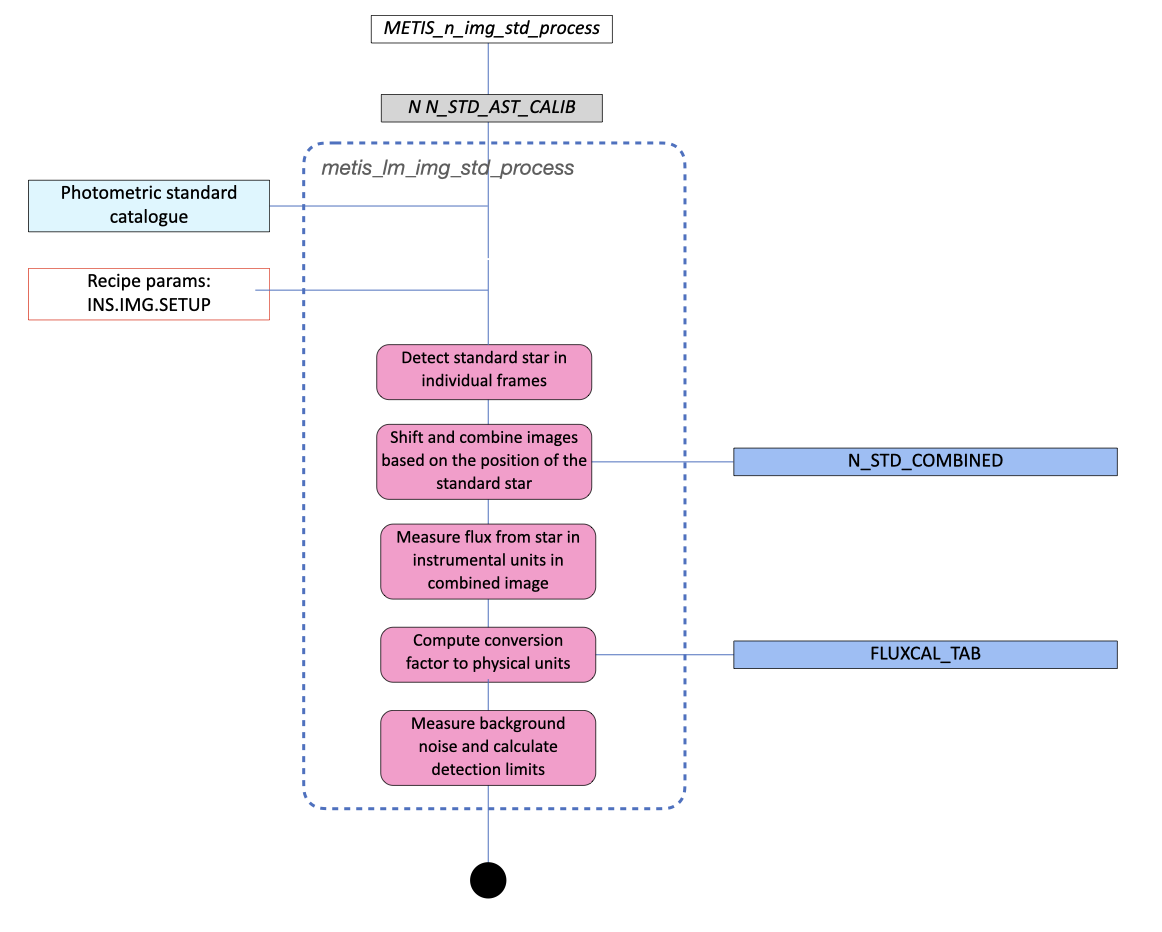
\includegraphics[width=0.6\textwidth]{lm_img_calibrate}
  \caption[Recipe: \REC{metis_lm_img_calibrate}]{\REC{metis_lm_img_calibrate} --
    Convert images to physical flux units and update FITS header}
  \label{fig:metis_lm_img_calibrate}
\end{figure}


%%%%%%%%%%%%%%%%%%%%%%%%%%%%
\clearpage
\subsubsection{LM-band imaging post-processing}
\label{lm_img_postprocess}
\label{rec:lm_img_postprocess}
\label{sssec:lm_img_postprocess}

This recipe coadds a sequence of flux-calibrated,
background-subtracted images (possibly from several observing blocks)
after resampling the images on a common pixel grid defined by a
standard sky projection. The alignment of the images (\FITS{CRVAL}
keywords, rotation) may have to be checked and refined through
cross-correlation of the overlapping images (TBC). The number of input
images contributing to any pixel in the output image (variable due to
dither offsets and bad pixels) will be documented in a contribution
map.

This recipe will only be used in the science-grade pipelines, not at
the observatory.

\begin{recipedef}\label{rec:lm_img_flat}
  Name:                & \REC{metis_lm_img_sci_postprocess}                         \\
  Purpose:             & Coadd reduced images.                                      \\
  Requirements:        & \REQ{METIS-6104}                                           \\
  Templates:           & ---                                                        \\
  Type:                & Science                                                    \\
  Input data:          & Calibrated science images (\PROD{LM_SCI_CALIBRATED})       \\
                       & Associated bad-pixel maps (\PROD{BADPIX_MAP_2RG})           \\
  Parameters:          & None (TBD).                                                \\
  Algorithm:           & Check and refine WCS of input images by cross-correlation  \\
                       & \hspace{1em} (on object catalogue or on image).            \\
                       & Determine output pixel grid encompassing all input images. \\
                       & Resample images to output pixel grid.                      \\
                       & Coadd.                                                     \\
  Output data:         & \PROD{LM_SCI_COADD} (coadded, mosaiced image)              \\
                       & \PROD{LM_SCI_COADD_ERROR} (coadded, mosaiced error image)  \\
                       & \PROD{LM_SCI_COADD_CONTRIB} (contribution map)             \\
  Expected accuracies: & TBD                                                        \\
  QC1 parameters:      & \QC{QC LM SCI NEXPOSURE}                                   \\
\end{recipedef}

\begin{figure}[hb]
  \centering
  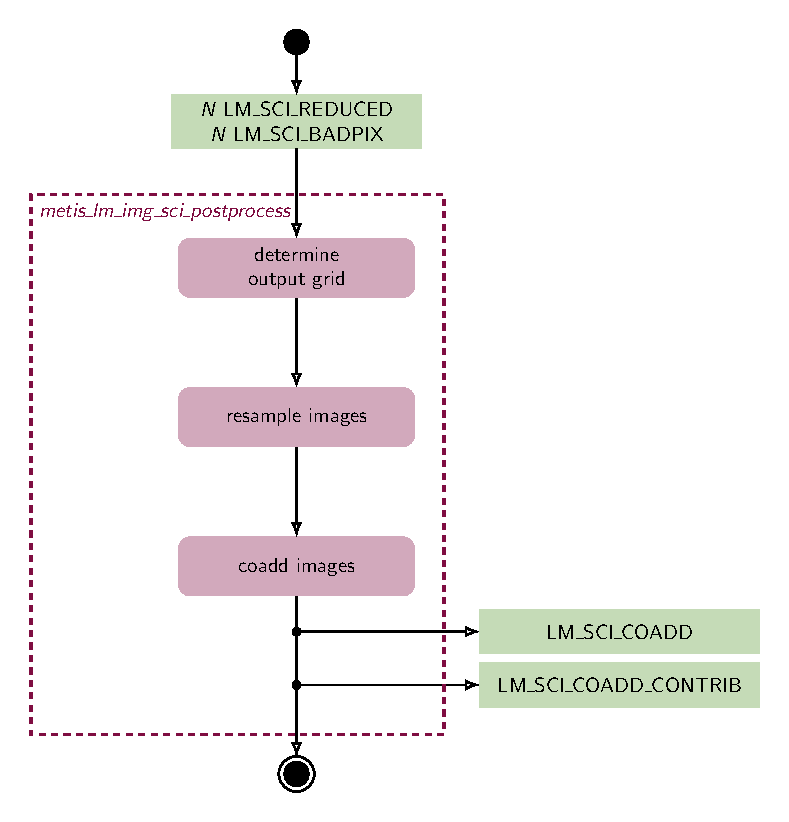
\includegraphics[width=0.7\textwidth]{metis_lm_img_sci_postprocess}
  \caption[Recipe: \REC{metis_lm_img_sci_postprocess}]{%
    \REC{metis_lm_img_sci_postprocess} -- post-processing (coaddition)
    of reduced \CODE{IMG_LM} science frames.}
  \label{fig:metis_lm_img_sci_postprocess}
\end{figure}

%%%%%%%%%%%%%%%%%%%%%%%%%%%%%%%%%%%%%%%%%%%%
\clearpage
\subsubsection{LM-band imaging distortion calibration}
\label{lm_img_distortion}
\label{rec:lm_img_distortion}
\label{sssec:lm_img_distortion}

Calibration of the imaging distortion is done on an image of a
pin-hole grid mask located in a focal plane within the instrument. The
distortion is described in terms of a polynomial model whose
coefficients can be transformed to WCS keywords and applied to any
other pipeline product. In addition to the distortion table, a map of
pixel scale across the detector will be created.

\begin{recipedef}
  Name:                & \REC{metis_lm_img_distortion}                                   \\
  Purpose:             & Determine optical distortion coefficients for the LM imager.    \\
  Requirements:        & \REQ{METIS-6087}                                                \\
  Templates:           & \TPL{METIS_img_lm_cal_distortion}                               \\
  Type:                & Calibration                                                     \\
  Input data:          & Images of grid mask in WCU-FP2 or CFO-FP2.                      \\
                       & Image with WCU window closed (background)                       \\
                       & Grid of pinhole mask positions \\
                       & Bad pixel map                                                  \\
  Parameters:          & Parameters for fitting routine      \\
                       & \TBD \\
  Algorithm:           & Subtract background image.    (\CODE{hdrl_imagelist_sub_image})                                  \\
                       & Measure location of point source images in frames (\CODE{hdrl_catalogue_create})             \\
                       & call \hyperref[drl:fit_distortion]{\CODE{fit_distortion}} to fit polynomial coefficients to deviations from grid positions.  \\
  Output data:         & \hyperref[dataitem:lm_distortion_table]{\PROD{LM_DISTORTION_TABLE}} \\
                       & \hyperref[dataitem:lm_distortion_map]{\PROD{LM_DISTORTION_MAP}}        \\
                       & \hyperref[dataitem:lm_dist_reduced]{\PROD{LM_DIST_REDUCED}}               \\
  Expected accuracies: & TBD                                                             \\
  QC1 parameters:      & \hyperref[qc:qc_lm_distort_rms]{\QC{QC LM DISTORT RMS}}                                          \\
                       & \hyperref[qc:qc_lm_distort_nsource]{\QC{QC LM DISTORT NSOURCE}}  \\
  hdrl functions:      & \CODE{hdrl_catalogue_create}                                    \\
                       & \CODE{hdrl_imagelist_sub_image}                                \\
\end{recipedef}

\begin{figure}[hb]
  \centering
  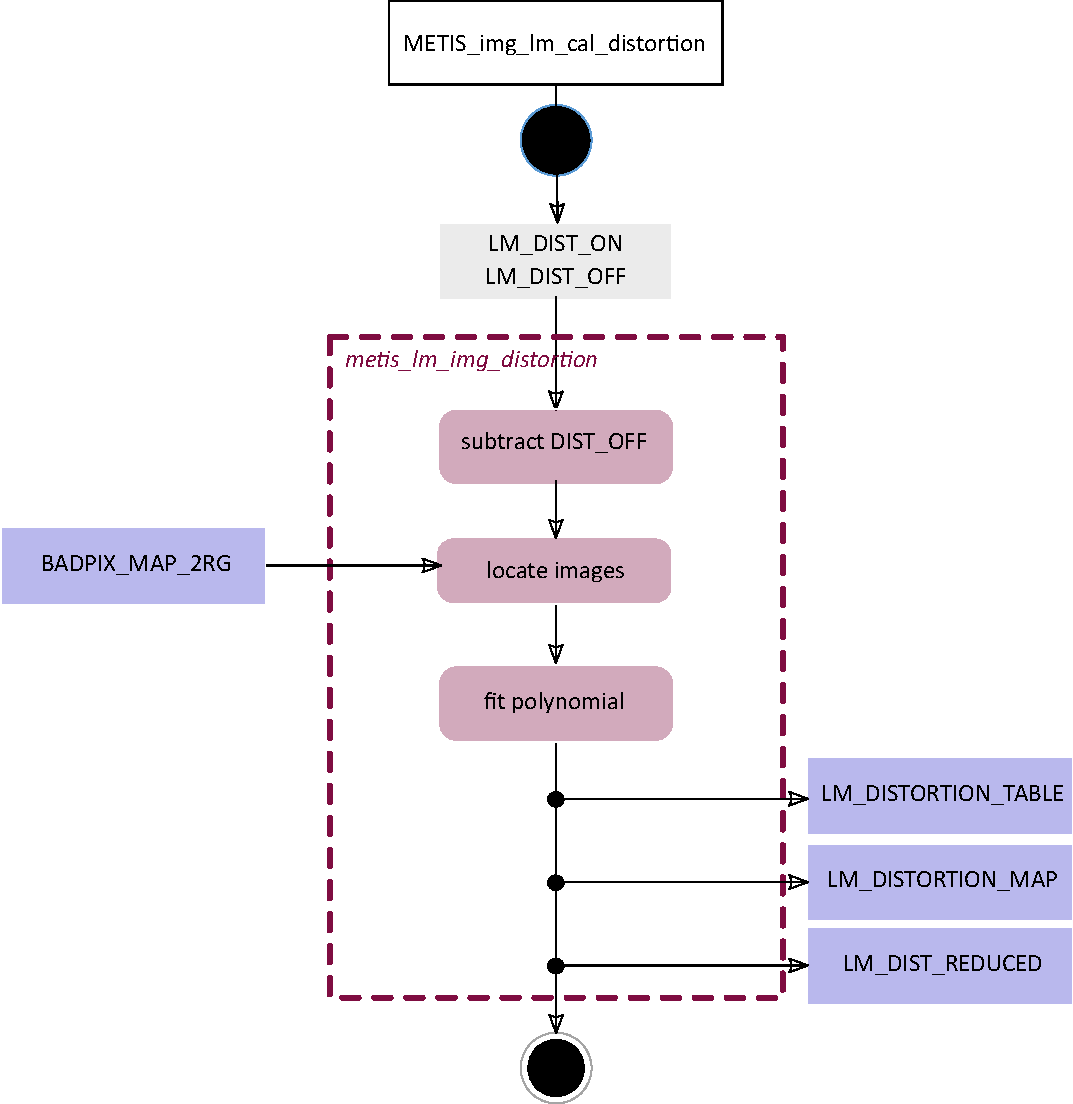
\includegraphics[width=0.6\textwidth]{metis_lm_img_distortion}
  \caption[Recipe: \REC{metis_lm_img_distortion}]{%
    \REC{metis_lm_img_distortion} -- LM IMG distortion calibration}
  \label{fig:metis_lm_img_distortion}
\end{figure}

\FloatBarrier

%%% Local Variables:
%%% TeX-master: "METIS_DRLD"
%%% End:
